% =====================================================================
\section{Diseño de la estación de carga}
\label{sec:diseno}

\subsection{Características del caso}
\begin{table}[H]
\centering\small
\caption{Datos generales del caso.}\label{tab:sitio}
\begin{tabularx}{\textwidth}{L{4.2cm}Y}
\toprule
Ubicación & Parqueo norte del campus Sede Central de la UTN, Villa Bonita, Alajuela (unos 960~msnm). Coordenadas de la estación: 10,0065\,°N; 84,2155\,°O (imagen satelital, $\pm$10~m).\\
Propietario y operador & Universidad Técnica Nacional (catastro A-652521-2000); se propone que la opere la UTN con el TEC como usuario institucional.\\
Uso & Público con acceso controlado: estudiantes, personal y visitantes del campus. Permanencia típica de 2 a 9~h en CA y de menos de 1~h en CC.\\
Vehículos que se atienden & Flota mixta del país: GB/T (BYD), J1772/CCS1 (mercado estadounidense), CHAdeMO (Leaf usados) y NACS con adaptador (Tesla).\\
Alimentación & Transformador del ICE N.\textsuperscript{o} 119688, 750~kVA, 34,5~kV/480Y/277~V (E01, Proyecto~2). Servicio nuevo de 480Y/277~V, 3F 4H.\\
Fuentes del sitio & Imagen satelital Esri World Imagery z19 (1/11/2026) \cite{esri}, lámina E01 as-built, unifilar E07 y registro fotográfico del 5/10/2026 (Proyecto~2) \cite{p2}.\\
\bottomrule
\end{tabularx}
\end{table}

\begin{figure}[htbp]
\centering
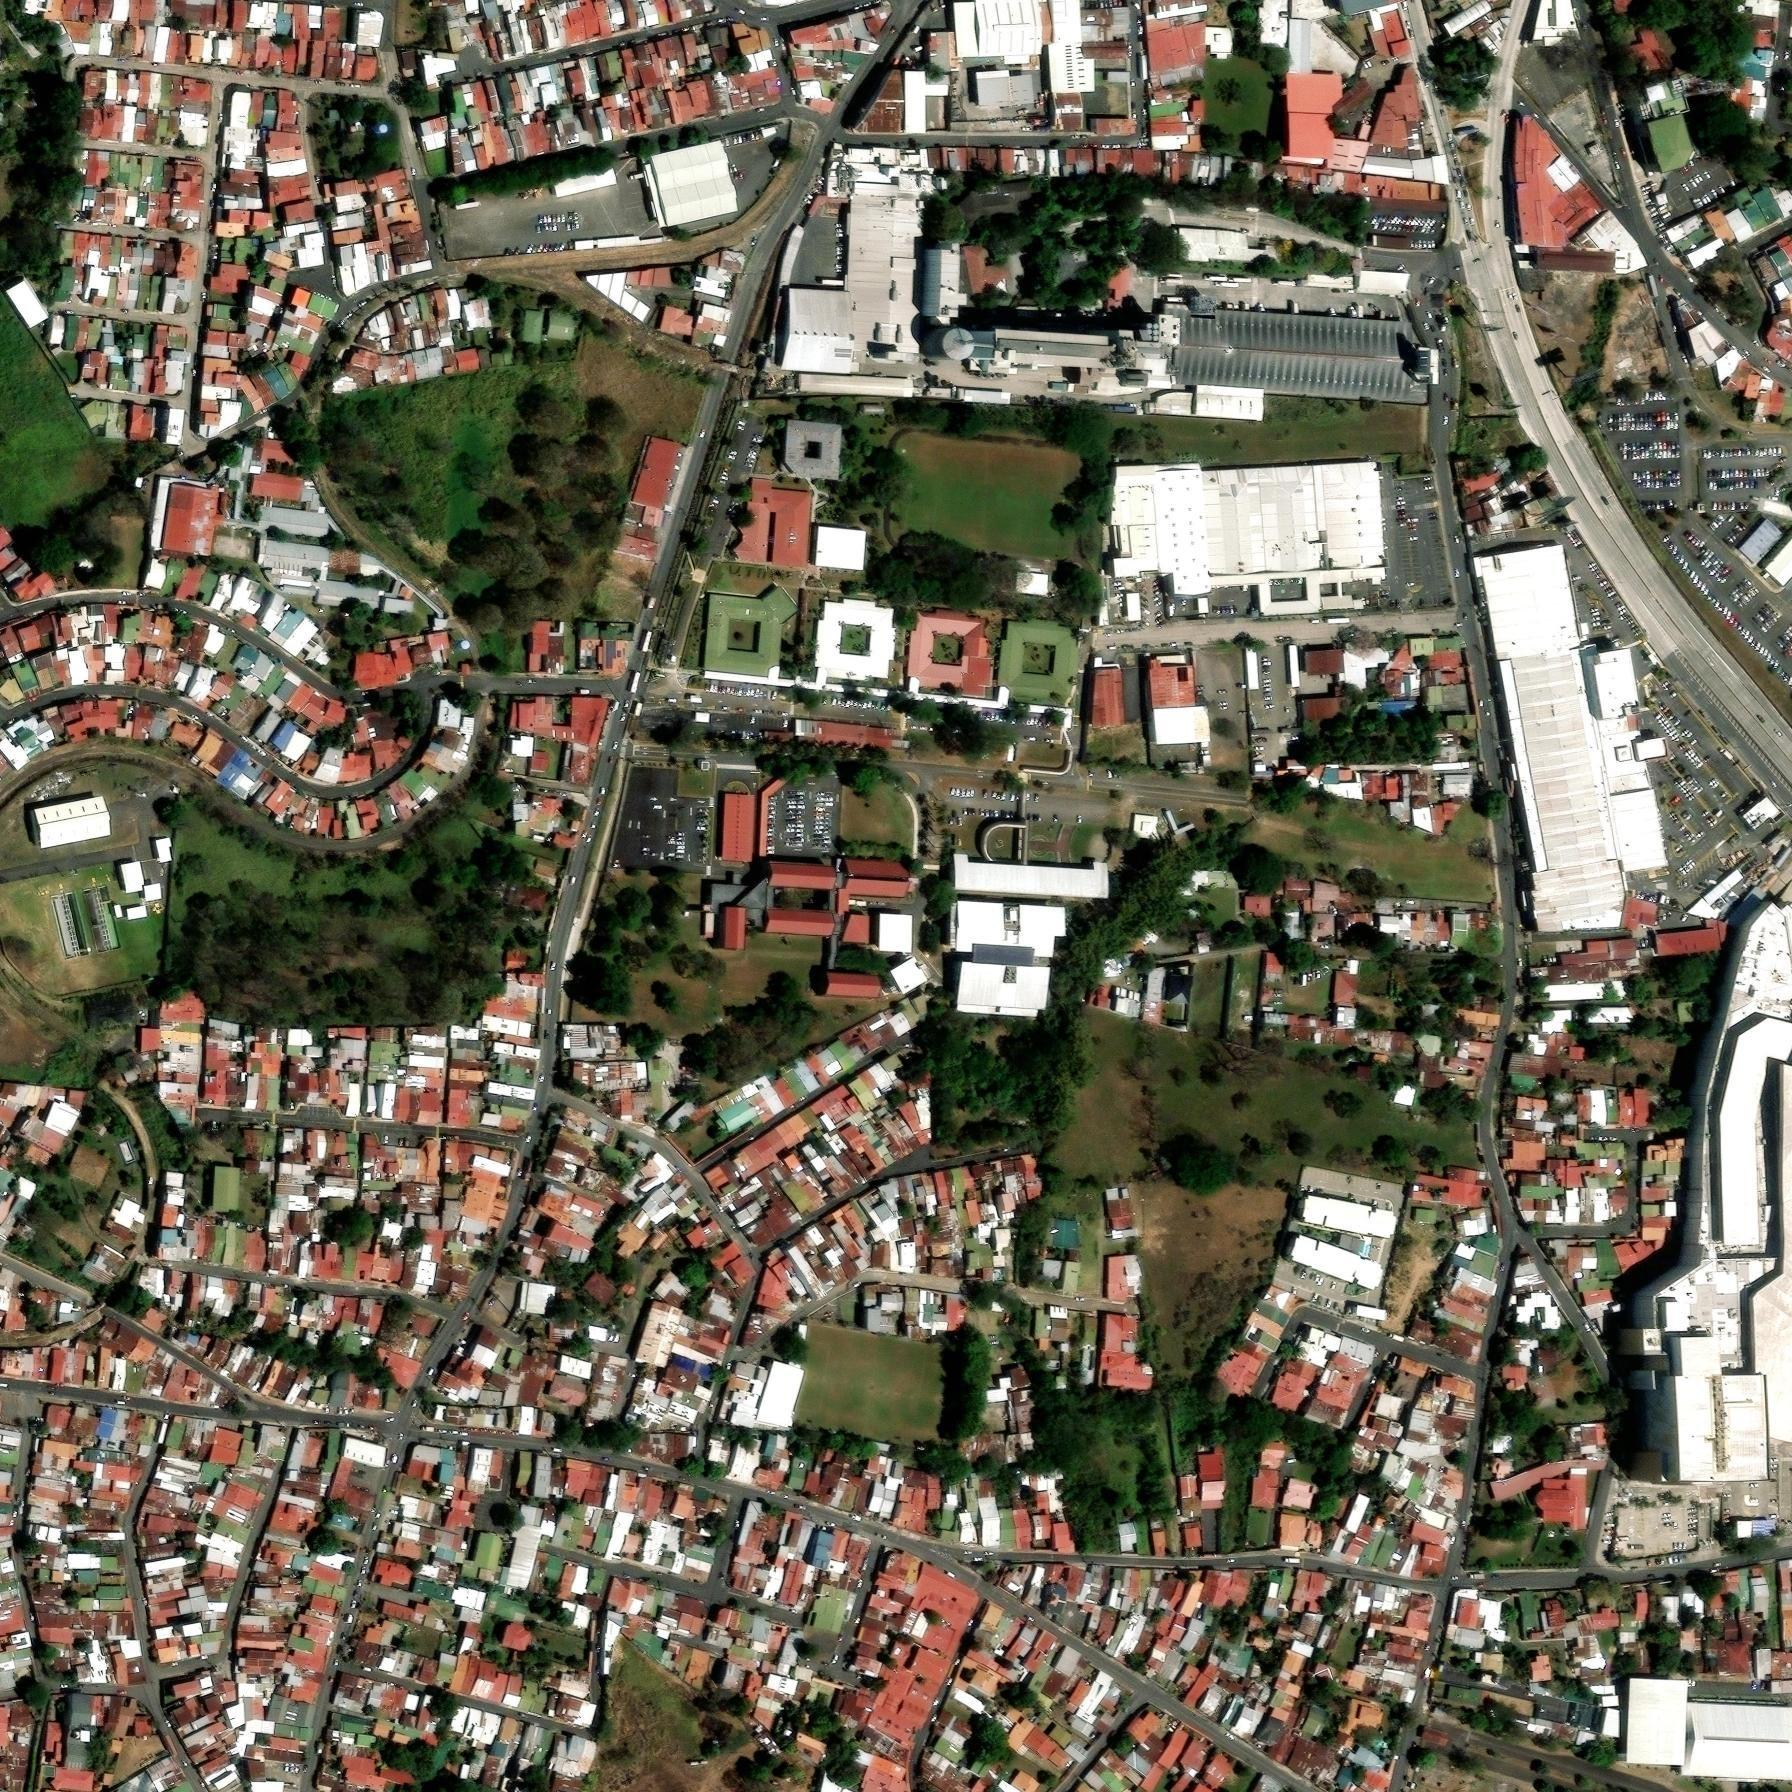
\includegraphics[width=0.85\textwidth]{figuras/satelital_campus_z18.jpg}
\caption{Imagen satelital del campus UTN Villa Bonita (Esri World Imagery, nivel 18, 0,59~m por píxel, descargada el 1/11/2026). El CAA-TEC es el edificio blanco girado junto a los techos rojos; el parqueo norte está entre la calle interna y la plaza del arco.}
\label{fig:satelital}
\end{figure}

\textbf{Por qué este sitio.} Es el mismo campus del Proyecto~2, así que se conocen el transformador, la medición, la malla de tierra y la ruta de la acometida existente, verificados en sitio. El parqueo ya existe y tiene una franja verde al sur, donde caben la isla de cargadores y la celda eléctrica sin quitar circulación. Está a menos de 120~m del transformador y la ruta del alimentador evita edificios y árboles (lámina VE-00).

{\small
\begin{longtable}{L{3.3cm}L{5.4cm}L{6.3cm}}
\caption{Supuestos de diseño (marcados con \supuesto{} en el texto).}\label{tab:supuestos}\\
\toprule
\textbf{Dato} & \textbf{Valor adoptado y fundamento} & \textbf{Efecto si el valor real difiere}\\
\midrule\endfirsthead
\toprule
\textbf{Dato} & \textbf{Valor adoptado y fundamento} & \textbf{Efecto si el valor real difiere}\\
\midrule\endhead
Capacidad remanente del transformador 119688 & $\ge$ 100~kVA. El CAA demanda unos 110~kVA (P2); el resto de las cargas de la UTN se desconoce & Si es menor, el EMS puede bajar el límite (por ejemplo, a 40~kW) o el ICE cambia el transformador. Lo define el estudio de capacidad.\\
Impedancia del transformador & 5,75\,\%, X/R = 5 (valor típico de 750~kVA) & Con 4,5\,\%, la corriente de falla sube a unos 20~kA, todavía menor que los 35~kA de IP-VE.\\
Posición del nicho y longitud del alimentador & Según E01; ruta medida de unos 111~m; se adoptan 120~m & Con 150~m, la caída sube a 1,9\,\% con \#3/0; sigue cumpliendo.\\
Impedancia de T-VE & 4,5\,\% & Corriente de falla en TD-AC de 2,8~kA o menos, frente a 10~kA de capacidad.\\
Temperatura ambiente & 31--35~°C (factor 0,96), como en P2 & Conservador para el Valle Central.\\
Eficiencias de carga & CA red--batería 0,90; cargador CC 0,95; vehículo en CC 0,97 & $\pm$5\,\% en energía y tiempo.\\
Curvas de aceptación en CC & Forma típica con el máximo del fabricante (\texttt{calc/carga.py}) & El tiempo del 20 al 80\,\% depende poco de ellas porque DC-1 limita a 60~kW.\\
Capacidades útiles & Leaf 39~kWh y Model Y 75~kWh (no publicadas como ``útiles'') & Proporcional en energía y tiempo.\\
Escenario de uso & 14 sesiones por día lectivo, 250 días lectivos y 115 días con 30\,\% del uso & Con la mitad del uso, el costo por kWh sube (sección~\ref{sec:economia}).\\
Espacios & 2,50~m $\times$ 5,00~m como base, ensanchados a 2,6--2,8~m; accesible de 3,30~m $\times$ 5,00~m & Confirmar con el reglamento de construcciones y el de la Ley 7600.\\
Precios sin cotización & Estimaciones de mercado (Cuadro~\ref{tab:bom}); tipo de cambio de ₡505/USD & El presupuesto puede variar $\pm$20\,\%.\\
Iluminación & 50~lx medios en la zona de conexión & Confirmar con INTE N121.\\
\bottomrule
\end{longtable}}

\subsection{Criterios de diseño}
\begin{enumerate}[leftmargin=1.2cm]
\item Atender la flota real del país sin depender de adaptadores no aprobados: J1772, GB/T, CCS1 y CHAdeMO.
\item Dar carga lenta en CA a quien permanece varias horas (la mayoría de los usuarios del campus) y carga rápida en CC a visitantes y a quien necesita autonomía inmediata.
\item Usar un servicio propio con medición independiente del CAA, para aplicar la tarifa correcta y, si se decide, vender el servicio (Ley 10937).
\item Seleccionar equipos listados (UL) cuando existan. Si no existen (GB/T), documentar la evaluación de la conformidad y agregar protección.
\item Considerar todas las cargas como continuas (125\,\%), con caída de tensión de 3\,\% o menos por tramo y de 5\,\% o menos en total.
\item Limitar la demanda con un EMS para reducir el cargo por demanda y el riesgo de capacidad.
\item Dejar previstos dos puntos de CA más y un segundo cargador de CC (ducto de reserva y espacios libres).
\end{enumerate}

\subsection{Puntos de carga: cantidad, tipo, potencia y ubicación}
\begin{table}[H]
\centering\small
\caption{Puntos de carga de la estación.}\label{tab:puntos}
\begin{tabularx}{\textwidth}{L{1.3cm}L{1.1cm}L{2.6cm}L{2.2cm}L{2.0cm}Y}
\toprule
\textbf{Punto} & \textbf{Espacio} & \textbf{Tipo y potencia} & \textbf{Conector} & \textbf{Equipo} & \textbf{Vehículos compatibles y justificación}\\
\midrule
AC-1 & P1 (accesible) & Modo 3, 208~V, 40~A, 8,3~kW & J1772 (Tipo 1) & Autel AC Elite & Leaf, Ioniq 5, F-150 y Tesla con adaptador. Espacio accesible (Ley 7600).\\
AC-2 & P2 & Modo 3, 208~V, 40~A, 8,3~kW & J1772 & Autel AC Elite & Igual que AC-1.\\
AC-3 & P3 & Modo 3, 208~V, 32~A, 6,7~kW & GB/T CA & MDAC 132EN K & BYD (CR) y otros GB/T. No hay alternativa en CC dentro de la estación.\\
AC-4 & P4 & Modo 3, 208~V, 32~A, 6,7~kW & GB/T CA & MDAC 132EN K & Igual que AC-3.\\
DC-1 & P5 y P6 & Modo 4, 60~kW (30 + 30~kW) & CCS1 (P5) y CHAdeMO (P6) & Autel DC Fast 60~kW & Ioniq 5, F-150, Tesla con adaptador CCS1 (P5); Leaf (P6).\\
\bottomrule
\end{tabularx}
\end{table}

La lámina VE-00 (Fig.~\ref{fig:ve00}) ubica la estación en el campus, junto con el transformador del ICE y la ruta del alimentador. La lámina VE-01 (Fig.~\ref{fig:ve01}) muestra a escala 1:100 los espacios, los cargadores, la celda eléctrica, los recorridos de las canalizaciones, los accesos, las cotas y la leyenda de símbolos.

\lamina{laminas/VE-00.pdf}{Lámina VE-00 (A3): plano general de ubicación sobre la imagen satelital del campus.}{fig:ve00}
\lamina{laminas/VE-01.pdf}{Lámina VE-01 (A3): planta de la estación a escala 1:100, con espacios, equipos, canalizaciones, accesos, cotas y leyenda.}{fig:ve01}

\subsection{Diagrama unifilar}
La lámina VE-02 (Fig.~\ref{fig:ve02}) muestra el sistema desde los bornes del transformador del ICE hasta cada cargador: tensiones, fases, circuitos, conductores, protecciones, medios de desconexión, medición (ICE y EMS) y puesta a tierra.

\lamina{laminas/VE-02.pdf}{Lámina VE-02 (A3): diagrama unifilar de la estación.}{fig:ve02}

\subsection{Energía, potencia efectiva y tiempo de carga}
\label{sec:calc_carga}
\textbf{Procedimiento} (\texttt{calc/carga.py}). La potencia que llega a la batería en cada instante es el mínimo de tres límites, afectado por las pérdidas:
\begin{equation}
P_{bat}(SOC)=\eta\cdot\min\Big(\underbrace{P_{EVSE}}_{\text{cargador}},\;\underbrace{P_{veh}(SOC)}_{\text{vehículo}},\;\underbrace{V_{sum}\,I_{max}}_{\text{suministro}}\Big)
\end{equation}
\begin{itemize}
\item En CA, $P_{veh}$ es la potencia del cargador a bordo (constante hasta el 95\,\% de SOC, con reducción posterior por el balanceo de celdas).
\item En CC, $P_{veh}$ es la curva de aceptación del vehículo, que baja con el SOC. Además, CHAdeMO está limitado a 125~A.
\end{itemize}
El tiempo se obtiene integrando el SOC sin suponer potencia constante, $t=\int_{SOC_0}^{SOC_1}E_u\,dSOC/P_{bat}(SOC)$, y la energía tomada de la red es $E_{red}=\int P_{red}\,dt$. Se distinguen la potencia en kW y la energía en kWh.

\textbf{Ejemplo manual (BYD Dolphin en AC-3, del 20 al 80\,\%).}
\begin{itemize}
\item Límites: el EVSE da $208\times 32=\SI{6.66}{\kilo\watt}$; el OBC, \SI{6.6}{\kilo\watt}. Gobierna el OBC: $P_{red}=\SI{6.6}{\kilo\watt}$ y $P_{bat}=0{,}9\times 6{,}6=\SI{5.94}{\kilo\watt}$.
\item Energía a la batería: $\Delta E=0{,}6\times 44{,}9=\SI{26.9}{\kilo\watt\hour}$.
\item Resultado: $t=26{,}9/5{,}94=\SI{4.54}{\hour}$ (4~h~32~min) y $E_{red}=26{,}9/0{,}9=\SI{29.9}{\kilo\watt\hour}$, que coinciden con el programa.
\end{itemize}
\textbf{Efecto de la tensión de 208~V.} Con 40~A, el Ioniq~5 recibe \SI{8.3}{\kilo\watt} a 208~V, frente a \SI{9.6}{\kilo\watt} a 240~V: el tiempo del 20 al 80\,\% pasa de unas 5~h~22~min a 6~h~12~min. Se acepta porque la permanencia típica en el campus supera las 6~h, y porque el servicio de la UTN es trifásico.

\begin{table}[H]
\centering\small
\caption{Energía, potencia y tiempo de carga del 20 al 80\,\% de SOC (\texttt{calc/carga\_out.txt}).}\label{tab:tiempos}
\begin{tabularx}{\textwidth}{L{3.6cm}L{3.7cm}rrrrY}
\toprule
\textbf{Vehículo} & \textbf{Punto} & \textbf{$E_{bat}$ (kWh)} & \textbf{$E_{red}$ (kWh)} & \textbf{$\bar P_{bat}$ (kW)} & \textbf{$P_{red,max}$ (kW)} & \textbf{Tiempo}\\
\midrule
BYD Dolphin & AC-3/AC-4 (GB/T) & 26,9 & 29,9 & 5,9 & 6,6 & 4~h~32~min\\
Nissan Leaf & AC-1/AC-2 & 23,4 & 26,0 & 5,9 & 6,6 & 3~h~56~min\\
Nissan Leaf & DC-1 CHAdeMO (solo) & 23,4 & 25,4 & 36,0 & 47,6 & 39~min\\
Nissan Leaf & DC-1 compartido & 23,4 & 25,4 & 28,3 & 31,6 & 50~min\\
Hyundai Ioniq 5 & AC-1/AC-2 & 46,4 & 51,6 & 7,5 & 8,3 & 6~h~12~min\\
Hyundai Ioniq 5 & DC-1 CCS1 (solo) & 46,4 & 50,4 & 58,2 & 63,2 & 48~min\\
Hyundai Ioniq 5 & DC-1 compartido & 46,4 & 50,4 & 29,1 & 31,6 & 1~h~36~min\\
Tesla Model Y & AC-1/AC-2 (adaptador) & 45,0 & 50,0 & 7,5 & 8,3 & 6~h~01~min\\
Tesla Model Y & DC-1 CCS1 (adaptador) & 45,0 & 48,8 & 58,2 & 63,2 & 46~min\\
F-150 Lightning ER & AC-1/AC-2 & 78,6 & 87,3 & 7,5 & 8,3 & 10~h~30~min\\
F-150 Lightning ER & DC-1 CCS1 (solo) & 78,6 & 85,3 & 58,2 & 63,2 & 1~h~21~min\\
F-150 Lightning ER & DC-1 compartido & 78,6 & 85,3 & 29,1 & 31,6 & 2~h~42~min\\
\bottomrule
\end{tabularx}
\end{table}

\textbf{Lectura de los resultados.}
\begin{itemize}
\item En CA el límite lo pone el OBC en el Leaf y el Dolphin (6,6~kW) y el EVSE a 208~V en los vehículos de 10,9 a 19,2~kW.
\item En CC, el límite de 60~kW de DC-1 gobierna los vehículos con curvas altas (Ioniq 5, F-150, Model Y), mientras que el Leaf queda limitado por su propia curva y por CHAdeMO.
\item Cargar del 20 al 100\,\% en CC es ineficiente: el Leaf tarda 1~h~27~min (frente a 39~min hasta el 80\,\%) y el Model Y, 1~h~20~min. Por eso DC-1 se configura con un tope del 80\,\% para usuarios en espera.
\item La F-150 necesita 10~h~30~min en CA para recibir 78,6~kWh: para una pickup de batería grande en uso diario, el punto adecuado es DC-1.
\end{itemize}

\textbf{Escenario de uso y energía anual.} Con 14 sesiones por día lectivo (Cuadro~\ref{tab:supuestos}), la estación entrega 521~kWh a las baterías y toma 572~kWh de la red por día. DC-1 queda ocupado unas 5~h al día. Al año son \textbf{162,8~MWh} (81,5 en CA y 81,3 en CC), unos 13\,560~kWh al mes.

\subsection{Conductores, canalizaciones y caída de tensión}
\label{sec:cond}
\textbf{Procedimiento} (\texttt{calc/electrico.py}):
\begin{enumerate}
\item Corriente de diseño: $I_d=1{,}25\,I_{max}$ (625.41, 215.2).
\item Interruptor: el valor normalizado igual o siguiente (240.6).
\item Conductor con ampacidad $I_z=\min(I_{90}\,k_T\,k_A,\;I_{75})\ge I_d$, protegido por el interruptor (240.4(B)).
\item EGC según la Tabla 250.122.
\item Caída de tensión con la impedancia eficaz de la Tabla 9: $\Delta V=k\,I\,L\,(R\cos\phi+X\sin\phi)$, con $k=\sqrt3$ en circuitos trifásicos y $k=2$ en monofásicos.
\end{enumerate}

\begin{table}[H]
\centering\small
\caption{Dimensionamiento de conductores, protecciones y canalizaciones.}\label{tab:conductores}
\footnotesize\setlength{\tabcolsep}{3pt}
\begin{tabular}{L{1.5cm}R{1.0cm}R{1.0cm}L{1.9cm}L{3.0cm}R{0.9cm}R{0.7cm}R{0.9cm}L{2.7cm}}
\toprule
\textbf{Circuito} & \textbf{$I_{max}$ (A)} & \textbf{1,25$I$ (A)} & \textbf{OCPD (A)} & \textbf{Conductores Cu THWN-2} & \textbf{$I_z$ (A)} & \textbf{L (m)} & \textbf{$\Delta V$ (\%)} & \textbf{Tubo PVC-40 (ocupación)}\\
\midrule
AL-VE & 146,2 & 182,8 & 200, 3P & 3\#3/0 + N\#4 + EGC\#6 & 200 & 120 & 1,54 & 3'' (12,9\,\%) + reserva\\
DC-1 & 91,0 & 113,8 & 125, 3P & 3\#1 + EGC\#6 & 130 & 8 & 0,13 & 1-1/2'' (26,2\,\%)\\
T-VE prim. & 54,1 & 67,7 & 70, 3P & 3\#4 + EGC\#8 & 85 & 3 & -- & 1''\\
T-VE sec. & 124,9 & -- & 125 (TD-AC) & 3\#1 + N\#1 + EGC\#6 & 130 & $\le$3 & 0,13 & 1-1/2''\\
AC-1, AC-2 & 40 & 50 & 50, 2P & 2\#6 + EGC\#10 c/u & 57,6 & 18 & 1,12 & 1'' (26,9\,\%, 2 circ.)\\
AC-3, AC-4 & 32 & 40 & 40, 2P + RCD B & 2\#8 + EGC\#10 c/u & 42,2 & 13 & 1,02 & 1'' (20,1\,\%, 2 circ.)\\
Alumbrado & 1,1 & 1,4 & 20, 1P 277~V & 2\#12 + EGC\#12 & 25 & 40 & $<$0,5 & 3/4'' (7,9\,\%)\\
\bottomrule
\end{tabular}
\end{table}

\begin{itemize}
\item \textbf{Alimentador:} se dimensionó con la capacidad nominal completa de T-VE (54,1~A) para dejar prevista la ampliación de CA: $1{,}25\times(91+54{,}1+1{,}1)=\SI{182.8}{\ampere}$. Con la carga instalada real (129,3~A), la caída es de 1,54\,\%. Con \#2/0 sería de 1,97\,\%, pero su ampacidad (175~A) queda por debajo de 182,8~A, así que se descarta.
\item \textbf{Caída total:} 1,68\,\% hasta DC-1 y 2,79\,\% en el peor ramal de CA, dentro del criterio de 5\,\%.
\item \textbf{Canalizaciones:} todas subterráneas a 600~mm, con ocupación de 40\,\% o menos. Se usan tubos de 3'' en el alimentador para facilitar el halado de 120~m, más un ducto de reserva para un segundo cargador de CC.
\item \textbf{Balance de fases en 208~V:} A = 92,3~A, B = 98,3~A, C = 70,8~A. La fase más cargada al 125\,\% da 122,9~A, menor que el principal de 125~A de TD-AC.
\end{itemize}

\subsection{Protecciones, puesta a tierra y medios de desconexión}
\label{sec:cc}
\begin{itemize}
\item \textbf{Sobrecorriente:} las del Cuadro~\ref{tab:conductores}.
  \begin{itemize}
  \item T-VE se protege solo en el primario con 125\,\% o menos (70~A $\ge$ 67,7~A, permitido por la nota~1 de la Tabla 450.3(B)).
  \item Los conductores del secundario, de 3~m o menos, terminan en el principal de 125~A de TD-AC (240.21(C)(2)).
  \end{itemize}
\item \textbf{Capacidad interruptiva:} se calculó con barra infinita y $Z$ = 5,75\,\% \supuesto{}.
  \begin{itemize}
  \item $I_{cc}=\SI{15.7}{\kilo\ampere}$ en los bornes del transformador: IP-VE es un PowerPact J de 35~kA. El interruptor existente del CAA es de 18~kA.
  \item \SI{5.8}{\kilo\ampere} en TD-VE (tablero de 14~kA o más).
  \item \SI{2.8}{\kilo\ampere} en TD-AC (QO de 10~kA).
  \item DC-1 tiene un SCCR de 65~kA o más.
  \end{itemize}
  Los valores se rotulan en TD-VE (110.24).
\item \textbf{Falla a tierra y corrientes residuales:}
  \begin{itemize}
  \item AC-1/AC-2 llevan un CCID de 20~mA integrado (UL 2231).
  \item DC-1 tiene monitoreo de aislamiento (IMD), detección de falla a tierra y botón de emergencia.
  \item AC-3/AC-4 llevan, además de su protección interna contra fugas, un \textbf{diferencial tipo~B de 30~mA} aguas arriba. Así detectan fallas con componente continua que un diferencial tipo~A no ve (IEC 60364-7-722), y quedan cubiertos aunque no tengan listado UL.
  \end{itemize}
\item \textbf{Sobretensiones:} SPD tipo~1 en TD-VE, tipo~2 en TD-AC y los SPD internos de los cargadores.
\item \textbf{Puesta a tierra:} electrodo propio de dos varillas (250.32, 250.53) con GEC \#6. T-VE es un sistema derivado separadamente con puente N--T propio (250.30). En TD-VE el neutro y la tierra van separados. EGC continuo y unión de las partes metálicas (VE-03, D4).
\item \textbf{Desconexión:}
  \begin{itemize}
  \item IP-VE: desconectador del servicio en el nicho, rotulado.
  \item Principal de TD-VE con disparo en derivación, accionado por EPO-1 o EPO-2 (desenergiza toda la estación).
  \item Interruptor de DC-1 bloqueable en abierto (625.43).
  \item Interruptores de los ramales en TD-AC, a la vista de los pedestales.
  \end{itemize}
\item \textbf{Coordinación con las protecciones integradas:}
  \begin{itemize}
  \item Ante una sobrecarga o falla del lado del vehículo, actúan primero las protecciones internas del EVSE: los relés que abren el contactor y el CCID.
  \item Una falla interna del equipo la despeja su interruptor de ramal: 40/50~A frente a 125~A en TD-AC, y 125~A frente a 200~A en TD-VE.
  \end{itemize}
  La relación de corrientes nominales entre niveles es de 1,6 o más, lo que da selectividad en la zona de sobrecarga. En la zona instantánea no se garantiza, y el NEC no la exige en este tipo de instalación.
\end{itemize}

\subsection{Detalles de conexión y montaje}
La lámina VE-03 (Fig.~\ref{fig:ve03}) reúne los detalles:
\begin{itemize}
\item D1: pedestal de CA, con conector a 0,9--1,2~m, gestor de cable, dado de anclaje y bolardo.
\item D2: sección de la zanja, a 600~mm, con arena, cinta de advertencia y ducto de reserva.
\item D3: base de DC-1.
\item D4: puesta a tierra.
\item D5: rotulación (NEC 110.21, 110.24, 625.43, INTE N120 y Ley 7600).
\item D6: emergencia y mantenimiento.
\end{itemize}
Contra el agua, todo va sobre bases elevadas, con entrada de tubos por abajo y sellada. Contra el polvo y la corrosión, se usan equipos NEMA 3R/4 o IP54 y herrajes inoxidables. Contra los impactos, bolardos y topes. Los cables y conectores se manejan con gestores de cable y fundas.

\lamina{laminas/VE-03.pdf}{Lámina VE-03 (A3): detalles de montaje, zanja, puesta a tierra, rotulación, emergencia y mantenimiento.}{fig:ve03}

\subsection{Cuadro de cargas, cuadro de equipos y lista de materiales}
\begin{table}[H]
\centering\small
\caption{Cuadro de cargas (corriente máxima de entrada de cada equipo, NEC 625.42).}\label{tab:cargas}
\begin{tabularx}{\textwidth}{L{1.6cm}L{4.4cm}rrrrY}
\toprule
\textbf{Circuito} & \textbf{Carga} & \textbf{V} & \textbf{I (A)} & \textbf{kVA} & \textbf{Fases} & \textbf{Tablero / protección}\\
\midrule
DC-1 & Cargador rápido 60~kW & 480 & 91,0 & 75,7 & 3F & TD-VE, 3P 125~A\\
AC-1 & Cargador J1772 & 208 & 40 & 8,32 & A-B & TD-AC, 2P 50~A\\
AC-2 & Cargador J1772 & 208 & 40 & 8,32 & B-C & TD-AC, 2P 50~A\\
AC-3 & Cargador GB/T & 208 & 32 & 6,66 & C-A & TD-AC, 2P 40~A + RCD B\\
AC-4 & Cargador GB/T & 208 & 32 & 6,66 & A-B & TD-AC, 2P 40~A + RCD B\\
AUX & Tomacorriente, EMS, router, control & 120 & 8,3 & 1,00 & C & TD-AC, 1P 20~A\\
ILUM & 2 luminarias LED 150~W & 277 & 1,1 & 0,30 & -- & TD-VE, 1P 20~A\\
\midrule
\multicolumn{4}{l}{\textbf{Total instalado (sin EMS)}} & \textbf{107,0} & & demanda $\approx$ 94,5~kW\\
\multicolumn{4}{l}{\textbf{Límite con EMS (625.42)}} & & & 60~kW\\
\bottomrule
\end{tabularx}
\end{table}

\begin{table}[H]
\centering\small
\caption{Cuadro de equipos principales.}\label{tab:equipos}
\begin{tabularx}{\textwidth}{L{1.5cm}L{4.5cm}Y}
\toprule
\textbf{Código} & \textbf{Equipo (fabricante y modelo)} & \textbf{Especificación}\\
\midrule
DC-1 & Autel MaxiCharger DC Fast 60~kW, UF060A3001 & 480~V 3F, 91~A; CCS1 + CHAdeMO; UL 2202; NEMA 3R; OCPP\\
AC-1, AC-2 & Autel MaxiCharger AC Elite 50A, MC50AHS & 208~V, ajustado a 40~A; J1772 con 7,5~m; UL 2594; NEMA 4\\
AC-3, AC-4 & MDAC 132EN K, cabezal GB/T & 208~V entre fases, 32~A; GB/T; IP54; OCPP 1.6\\
T-VE & Transformador seco 45~kVA (Square D EE45T3H o equivalente) & 480$\Delta$--208Y/120~V; NEMA 3R; UL 1561\\
IP-VE & Schneider PowerPact JGL36200 en gabinete NEMA 3R & 200~A 3P, 480~V, 35~kA\\
TD-VE & Tablero 480Y/277~V, 225~A, principal de 200~A con disparo en derivación & NEMA 3R, 14~kA o más; SPD tipo 1\\
TD-AC & Square D QO, 208Y/120~V, 125~A, 24 espacios & NEMA 3R, 10~kA; SPD tipo 2\\
RCD-B & Diferencial tipo B 2P 40~A 30~mA & Para AC-3/AC-4\\
EMS & Controlador de gestión vía OCPP con TC en AL-VE & Límite de 60~kW\\
\bottomrule
\end{tabularx}
\end{table}

{\small
\begin{longtable}{L{1.4cm}L{7.4cm}rL{0.8cm}rrL{0.9cm}}
\caption{Lista de materiales y presupuesto referencial (USD, sin IVA, \texttt{calc/economico.py}). F = fuente del precio (Autel: tienda del fabricante, 1/11/2026; S: estimación de mercado).}\label{tab:bom}\\
\toprule
\textbf{Código} & \textbf{Descripción} & \textbf{Cant.} & \textbf{Ud.} & \textbf{P. unit.} & \textbf{Subtotal} & \textbf{F}\\
\midrule\endfirsthead
\toprule
\textbf{Código} & \textbf{Descripción} & \textbf{Cant.} & \textbf{Ud.} & \textbf{P. unit.} & \textbf{Subtotal} & \textbf{F}\\
\midrule\endhead
DC-1 & Autel MaxiCharger DC Fast 60~kW UL, CCS1 + CHAdeMO & 1 & u & 28\,000 & 28\,000 & S\\
AC-1/2 & Autel MaxiCharger AC Elite 50~A cableado, J1772 7,5~m & 2 & u & 639 & 1\,278 & Autel\\
AC-3/4 & Cargador CA GB/T 7~kW 32~A, IP54, OCPP 1.6 & 2 & u & 650 & 1\,300 & S\\
PED & Pedestal metálico doble con soporte de cable & 2 & u & 450 & 900 & S\\
RCD-B & Diferencial tipo B 2P 40~A 30~mA & 2 & u & 280 & 560 & S\\
T-VE & Transformador seco 45~kVA 480$\Delta$--208Y/120~V NEMA 3R & 1 & u & 5\,200 & 5\,200 & S\\
IP-VE & Interruptor 200~A 3P 35~kA en gabinete NEMA 3R & 1 & u & 2\,600 & 2\,600 & S\\
TD-VE & Tablero 480Y/277~V 225~A con principal de 200~A y disparo en derivación & 1 & u & 4\,800 & 4\,800 & S\\
INT-480 & Interruptores 3P 125~A, 3P 70~A y 1P 20~A 277~V & 1 & lote & 1\,620 & 1\,620 & S\\
TD-AC & Tablero QO 125~A 24 espacios con interruptores & 1 & u & 1\,000 & 1\,000 & S\\
SPD & Supresores tipo 1 y tipo 2 (UL 1449) & 1 & lote & 1\,300 & 1\,300 & S\\
EPO & Botones de paro de emergencia con rótulo & 2 & u & 250 & 500 & S\\
C-3/0 & Cu THWN-2 3/0 (3 $\times$ 126~m) & 378 & m & 14,0 & 5\,292 & S\\
C-4/6 & Cu THWN-2 \#4 (neutro) y \#6 (EGC) & 252 & m & 3,8 & 958 & S\\
C-RAM & Conductores de ramales & 1 & lote & 950 & 950 & S\\
PVC-3 & PVC cédula 40 de 3'' (alimentador + reserva) & 252 & m & 6,5 & 1\,638 & S\\
PVC-R & PVC de 3/4'' a 1-1/2'' y accesorios & 1 & lote & 650 & 650 & S\\
ZANJA & Zanja de 0,6~m con corte y reposición de asfalto & 125 & m & 45 & 5\,625 & S\\
REG & Registros de 60$\times$60~cm con tapa de tránsito & 5 & u & 350 & 1\,750 & S\\
BASES & Bases de concreto y anclajes & 1 & lote & 2\,500 & 2\,500 & S\\
BOL & Bolardos de acero rellenos de concreto & 10 & u & 180 & 1\,800 & S\\
TOPE & Topes de rueda & 6 & u & 60 & 360 & S\\
LUM & Postes de 6~m con luminaria LED de 150~W & 2 & u & 1\,400 & 2\,800 & S\\
PAT & Puesta a tierra (varillas, \#4 desnudo, soldadura) & 1 & lote & 600 & 600 & S\\
SEÑAL & Demarcación y rótulos (INTE N120, Ley 7600, NEC) & 1 & lote & 1\,200 & 1\,200 & S\\
MED & Medición indirecta del ICE y aporte de conexión & 1 & lote & 2\,500 & 2\,500 & S\\
MO & Mano de obra eléctrica y civil & 1 & lote & 9\,000 & 9\,000 & S\\
PEM & Puesta en marcha, OCPP, módem 4G, capacitación & 1 & lote & 1\,500 & 1\,500 & S\\
ING & Diseño, planos, CFIA, dirección técnica y permisos & 1 & lote & 5\,000 & 5\,000 & S\\
\midrule
 & \textbf{Subtotal} & & & & \textbf{93\,181} & \\
 & Imprevistos (10\,\%) & & & & 9\,318 & \\
 & \textbf{Total (unos ₡51,8 millones a ₡505/USD)} & & & & \textbf{102\,499} & \\
\bottomrule
\end{longtable}}

\subsection{Consumo y costo de operación}
\label{sec:economia}
Con 162,8~MWh al año y la demanda máxima mensual de la estación, el costo anual (\texttt{calc/economico.py}) incluye la energía, la demanda (12 meses) y la operación y mantenimiento: USD~3300 al año, que cubren el contrato de DC-1, el mantenimiento de la obra, la plataforma OCPP, la conectividad y la póliza de la Ley 10937.

\begin{table}[H]
\centering\small
\caption{Costo anual de operación según la tarifa y la gestión de carga (millones de colones, sin impuestos).}\label{tab:operacion}
\begin{tabularx}{\textwidth}{L{3.2cm}L{2.0cm}rrrrY}
\toprule
\textbf{Tarifa ICE 2026} & \textbf{Gestión} & \textbf{Energía} & \textbf{Demanda} & \textbf{O\&M} & \textbf{Total} & \textbf{₡/kWh (peso de la demanda)}\\
\midrule
T-CO & sin EMS (94,5~kW) & 9,71 & 11,18 & 1,67 & 22,56 & 138,6 (54\,\%)\\
T-CO & EMS 60~kW & 9,71 & 7,10 & 1,67 & 18,48 & 113,5 (42\,\%)\\
T-CS & sin EMS & 8,25 & 9,50 & 1,67 & 19,42 & 119,3 (54\,\%)\\
T-CS & EMS 60~kW & 8,25 & 6,04 & 1,67 & 15,96 & 98,0 (42\,\%)\\
\bottomrule
\end{tabularx}
\end{table}

El cargo por demanda es tan grande como el de energía porque DC-1 concentra hasta \SI{63}{\kilo\watt} en pocas horas al mes. El EMS reduce el costo anual entre ₡3,5 y ₡4,1 millones, con un costo casi nulo porque solo es configuración OCPP y un TC. Con precios iguales a los de la red pública (₡99,70/kWh en CA y ₡141/min en CC), los ingresos serían de unos ₡20,2 millones al año. La sección~\ref{sec:viabilidad} analiza el retorno.

\subsection{Funciones bidireccionales, fotovoltaica y almacenamiento}
La propuesta no incorpora carga entre vehículos, funciones bidireccionales, generación FV ni almacenamiento (sección~\ref{sec:bidir}), por lo que no requiere esquemas de flujo de energía adicionales. La razón principal es regulatoria: no hay un marco V2G aplicable ni equipos bidireccionales certificados disponibles. Hay además una razón económica: el cargo por demanda se controla más barato con el EMS que con una batería.

\subsection{Emergencia, mantenimiento, ampliación y cambios en la instalación existente}
\label{sec:ampliacion}
\begin{itemize}
\item \textbf{Emergencia:} dos EPO que abren TD-VE, el botón propio de DC-1, el procedimiento rotulado (VE-03, D6), un extintor y acceso libre para Bomberos por la calle interna. Ante un incendio de batería, el protocolo es desenergizar, aislar la zona y esperar a Bomberos.
\item \textbf{Mantenimiento:} el plan preventivo mensual, semestral y anual de VE-03. Para disponibilidad de repuestos se elige un solo fabricante principal (Autel) para los equipos UL, y se mantienen en sitio un conector J1772 y un cable CCS1.
\item \textbf{Ampliación:}
  \begin{itemize}
  \item T-VE (45~kVA, 69\,\% de uso) y TD-AC (dos espacios 2P de reserva) admiten dos puntos de CA más.
  \item TD-VE tiene un espacio 3P de reserva y existe un ducto de 3'' de reserva para un segundo cargador de CC. Ese cargador requiere aumentar IP-VE y el alimentador, o reducir la potencia con el EMS, y un nuevo estudio de capacidad del ICE.
  \item Una batería estacionaria o un sistema FV en el servicio de la estación reducirían la demanda facturada.
  \end{itemize}
\item \textbf{Cambios en la instalación existente:} la única intervención sobre la infraestructura actual es la conexión del servicio nuevo en el nicho del transformador 119688 (medición y IP-VE), que hace o autoriza el ICE. No se modifican el servicio, el TS-01 ni el TP del CAA. En el parqueo se pierden seis espacios de uso general, que pasan a ser exclusivos para VE, y se construye la isla sobre la franja verde existente.
\end{itemize}
